% Created 2023-06-05 Mon 18:33
% Intended LaTeX compiler: pdflatex
\documentclass[11pt]{article}
\usepackage[utf8]{inputenc}
\usepackage[T1]{fontenc}
\usepackage{graphicx}
\usepackage{grffile}
\usepackage{longtable}
\usepackage{wrapfig}
\usepackage{rotating}
\usepackage[normalem]{ulem}
\usepackage{amsmath}
\usepackage{textcomp}
\usepackage{amssymb}
\usepackage{mhchem}

\author{Eric Viklund}
\date{\date}
\title{Analysis of Niobium Electropolishing Using a Generalized Distribution of Relaxation Times Method}


\begin{document}


\maketitle
\tableofcontents


\section{Abstract}
\label{sec:org4ffe8c0}
\textbf{Using} electrochemical impedance spectroscopy, we have devised a method of sensing the microscopic surface conditions on the surface of niobium as it is undergoing an electrochemical polishing (EP) treatment. The method uses electrochemical impedance spectroscopy (EIS) to gather information on the surface state of the electrode without disrupting the polishing reaction. The EIS data is analyzed using a so-called distribution of relaxation times (DRT) method. Using DRT, the EIS data can be deconvolved into discrete relaxation time peaks without any apriori knowledge of the electrode dynamics. By analyzing the relaxation time peaks, we are able to distinguish two distinct modes of the EP reaction. As the polishing voltage is increased, the electrode transitions from the low voltage EP mode, characterized by two relaxation time peaks, to the high voltage EP mode, characterized by three relaxation time peaks. By analyzing EPed samples, we show that samples polished in the low voltage mode have significantly higher surface roughness due to grain etching and faceting. Samples polished in the high voltage mode obtain a smooth surface finish. This shows that EIS combined with DRT analysis can be use to predict etching on EPed Nb. This method can also be performed before or during the EP, which could allow for adjustment of polishing parameters to guarantee a smooth cavity surface finish.

\section{Introduction}
\label{sec:org5ef967f}
Electropolishing (EP) is commonly used to polish Nb SRF cavities to nanometer scale surface roughness. 

EIS has been used to study the chemistry of niobium in HF electrolytes before\ref{tian_2008,ranjith2018anodic,cattarin2002nb}. However, these studies have only analyzed the spectrum using qualitative methods or traditional equivalent circuit fitting techniques. These methods have proven insufficient for explaining several important phenomenon of EP such as surface etching and spontaneous current oscillations.

In this study, we use a model-free method of analyzing the EIS spectrum called distribution of relaxation times (DRT) analysis. The advantage of this method is that the EIS spectrum can be easily characterized over a large range of polishing conditions without making any assumptions about the underlying chemical processes. 

Using this method, we are able to observe the formation of the Nb\textsubscript{2}O\textsubscript{5} layer as the polishing voltage is increased. We also show that the formation of the oxide corresponds with a reduction in surface etching by analyzing Nb samples using SEM and confocal laser microscopy.


\section{Experimental}
\label{sec:orgb71f960}

A strip of Nb foil was prepared by cleaning with alcohol. A Nb wire was used as a pseudo-electrode, since it is resistant to the EP electrolyte. The counter electrode is an aluminum rod.

The EIS measurements were performed using a BioLogic VSP-300 potentiostat.



\section{Results}
\label{sec:org4a45003}

EIS measurements reveal a complex evolution of the surface chemistry as the polishing voltage is increased through the 0.5 V to 1.0 V range. As shown in \ref{fig:nyquistplot}, at 0.5 V the system exhibits a single capacitive process. This is most likely caused by the polarization of the electrical double-layer that occurs between the Nb electrode and the electrolyte. At this low voltage, the Nb\textsubscript{2}O\textsubscript{5} has not been formed due to the low oxidation current and high concentration of HF at the surface of the electrode.

When the voltage is increased, two new features appear, an inductive loop at mid-frequencies and a second capacitive loop at low frequencies. This low frequency loop as caused by the formation of the oxide film and depletion of the HF near the electrode surface. This limits the current through the electrode at higher voltages. 

When the voltage is increased from \qty{0.78}{\volt} to \qty{0.86}{\volt} the low frequency loop changes from decreasing impedance with increasing frequency to increasing as shown in \ref{fig:nyquistplot}.

\begin{figure}
  \label{fig:nyquistplot}
  
\includegraphics[]{figures/nyquist.png}
  \caption{The complex impedance of Nb. Each plot shows the different regimes of electropolishing at low voltage. A one capacitive loop, B two capacitive loops, C capacitive, inductive, and capacitive loops, D capacitive, inductive, and capacitive loop with a negative resistance.}
\end{figure}

The capacitive loop with increasing real impedance is indicative of a surface blocking process. This type of process is typically seen in electroplating processes containing a blocking species. This phenomenon is associated with brightening of the surface, since the blocking species preferentially blocks deposition on surface peaks.

For Nb electropolishing the blocking species is most likely niobium oxide, which limits the electrode reaction rate when the surface HF layer is depleted. The appearance of this low frequency impedance loop coincides with a significant change in the surface morphology of the electropolished Nb. The surface changes from an etched and facetted surface to a smooth surface at areound the same voltage as the low frequency loop appears. This is caused by the formation of the oxide film and depletion of the HF at the surface which makes the material removal rate more constant across the surface and eliminates any differences in surface energy caused by grain orientation.


\begin{figure}
    \label{fig:surface_maps}
    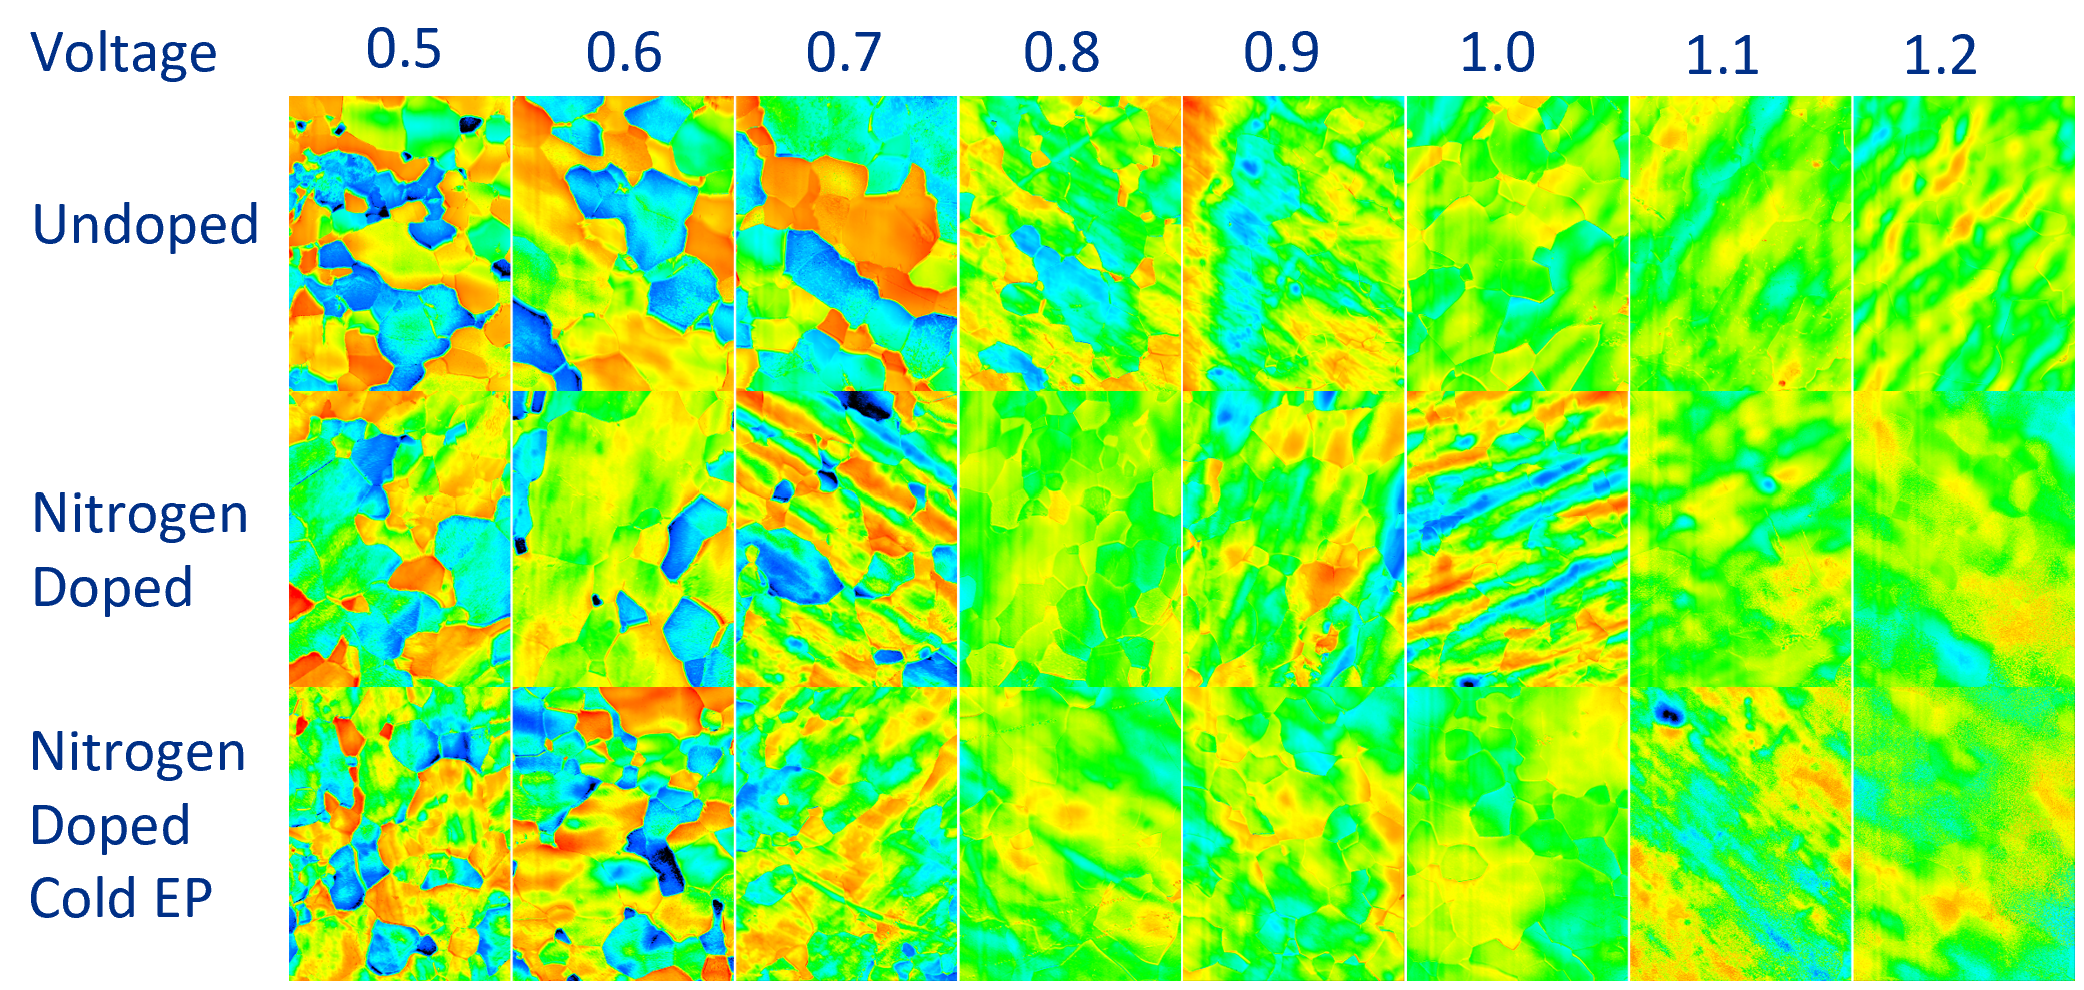
\includegraphics[]{figures/surface_maps.png}
    \caption{The surface height maps of Nb samples electropolished at different voltages and temperatures.}
\end{figure}






\section{Generalized Distribution of Relaxation Times}
\label{sec:org7d749e2}

The distribution of relaxation times is a flexible and general method that can be used to model complex impedance spectrum and extract useful information without the use of a pre-defined circuit model. In our study, we use this method to measure the changes on the niobium electrode as the polishing voltage is increased.

Traditional distribution of relaxation time analysis is based on an circuit model perspective on the electrochemical system. This perspective assumes the electrode is described by a series of voigt circuits, a resistor and a capacitor connected in parallel. By adding an infinite number of infinitesimal voigt elements, any arbitrary capacitive impedance can be described. The distribution of voigt elements is described by the distribution of relaxation times function.

\begin{flalign}
  \label{eq:Zrc}
  Z_{RC}&=\frac{R}{1+j\omega R C}\\
  Z_{DRT} &= R_{s} + \int_{0}^{\infty} \frac{G(\omega_0) d \omega_0}{1 + j \frac{\omega}{\omega_0}}
\end{flalign}

This model is sufficient to describe any capacitive-like processes with positive real impedance and negative imaginary impedance. However, this does not encompass all possible behaviors of electrochemical systems. The impedance of electrochemical systems can exist in all four quadrants of the complex impedance plane. For example, as seen in figure \ref{fig:nyquistplot}, for Nb electropolishing the low frequency impedance loop curls to the left at \qty{0.86}{\volt}. This impedance behavior can not be fitted by the traditional DRT method. The traditional method also can not fit inductive effects, which we measure during Nb EP. 

To explain these different behaviors it is more intuitive to abandon the circuit model perspective of the electrode and instead take a dynamical systems perspective. The electrochemical process can be described by a state vector and a system of first order differential equations that describe the evolution of the state vector over time. For a small perturbation near the steady state solution of this system, the impedance can be calculated as a sum of partial fractions.\cite{wu1998investigation, wu1999general}

\begin{flalign}
    \label{eq:gDRT}
    Z_{F} &= R_{t} + \sum_{i=1}^{n} \frac{k_{i}}{i \omega - s_{i}}
    Z_{gDRT} &= R_{t} + \int_{-\infty}^{\infty} \frac{k\left(s\right) ds}{i\omega - s}

\end{flalign}

If we let $s_{i} = \frac{1}{R_i C_i}$ and $k_{i} = \frac{1}{C_i}$ we see that this equation describes a voigt element. However, the dynamical systems approach does not assume that the impedance must follow the impedance of any real circuit elements. The constants $s_{i}$ and $k_{i}$ can take on both positive and negative values. If we perform the same procedure used to derive the DRT function for infinitesimal voigt elements, we arrive at the same expression with the only difference being the limits of integration span the entire real axis instead of just the positive real axis. The function $G\left(w_0\right)$ is also free to take both positive and negative values.

The mathematical derivation of the generalized DRT model is available in the supplemental section of this paper along with details on the numerical fitting method used to solve for the distribution of relaxation times.



\section{Distribution of Relaxation Times for Niobium Electropolishing}

Using the generalized DRT method, we are able to fit the Nb impedance spectrum across all frequencies including the inductive mid-frequency loop and the low frequency behavior as seen in figure \ref{fig:bodeplot}. Figure \ref{fig:gamma} shows distinct peaks in the relaxation time distribution which indicates that the model is not overfitting.

\begin{figure}
  \label{fig:bodeplot}
  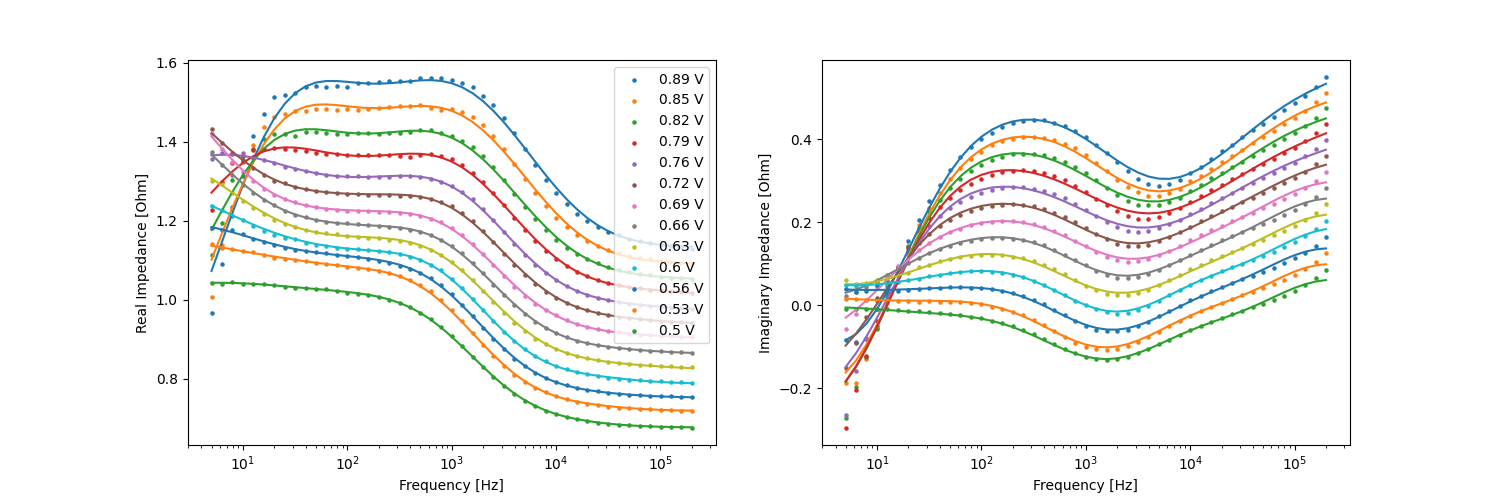
\includegraphics[]{figures/bodeplot.png}
  \caption{The complex impedance of Nb in electropolishing electrolyte measured using EIS. Each curve is offset from zero.}
\end{figure}

\begin{figure}
  \label{fig:gamma}
  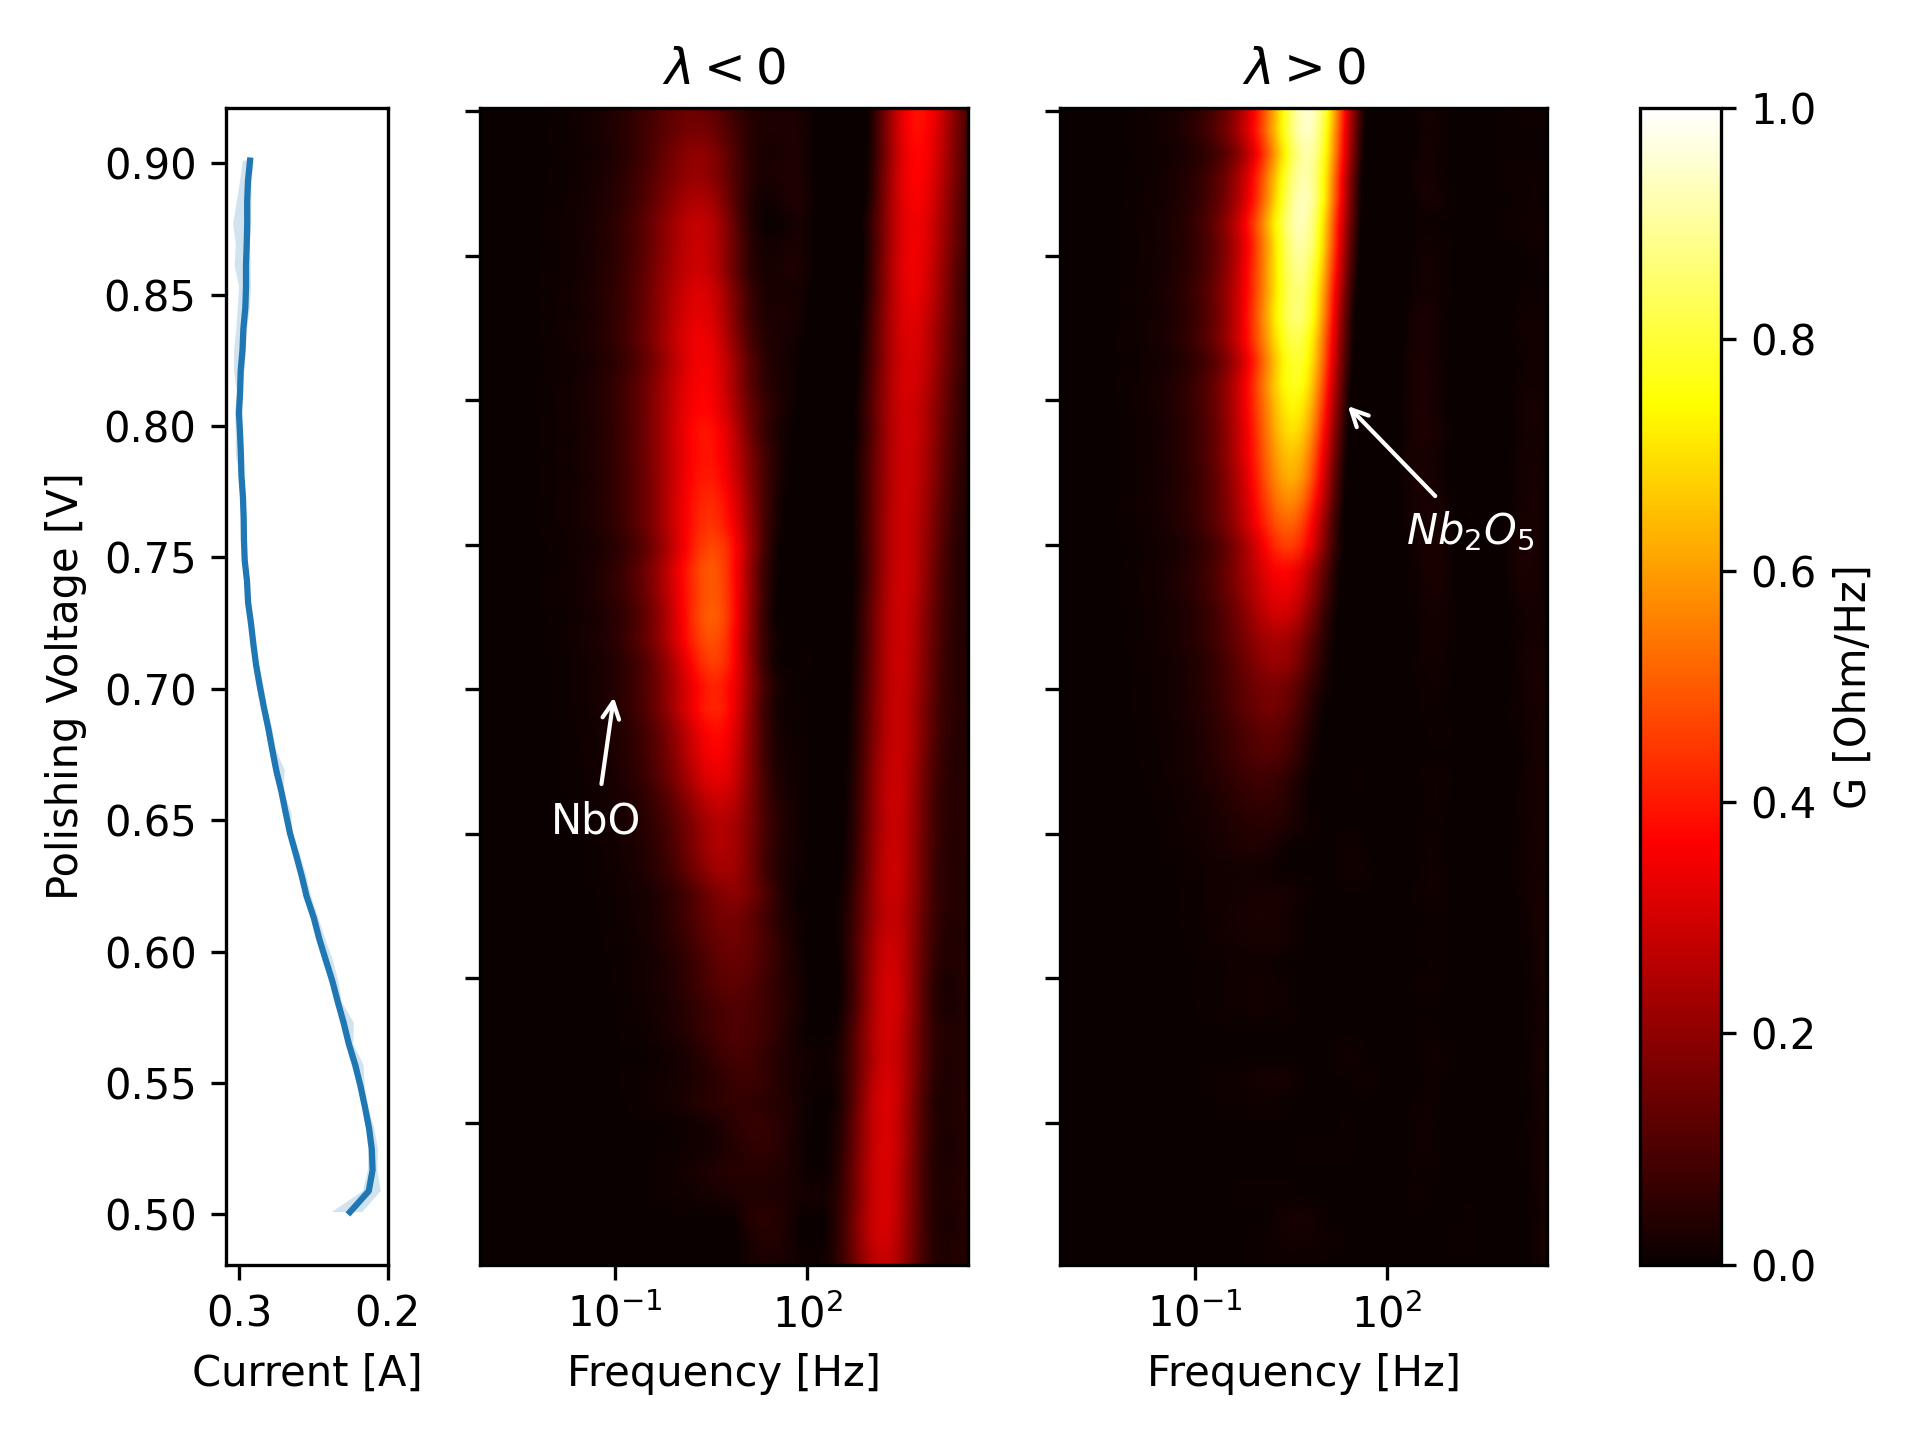
\includegraphics[]{figures/gamma.png}  
  \caption{The Distribution of relaxation times calculated from the EIS impedance data for each of the measured potentials. The current-voltage curve is shown in the graph on the left.}
\end{figure}

From figure \ref{fig:gamma} we can see that there are three promeinent peaks in the distribution of relaxations times. The peak centered around \qtyrange{100}{1000}{\hertz} corresponds to the electric double layer capacitance. The two other peaks centered around \qty{10}{\hertz} most likely correspond to the oxide layer. This low frequency peak gets more pronounced at higher voltages which indicates greater electrical impedance due to the oxide film. Around \qty{0.75}{\volts} the third peak appears in the negative \qty{10}{\hertz} region. This peak indicates that the oxide film is blocking the current flow leading to a negative current-voltage relationship.



\section{Discussion}

Comparing figure \ref{fig:gamma} to the electropolished samples shown in figure \ref{fig:surface_maps} we can see that the appearance of the third peak coincides with a significant change in the surface of the electropolished niobium. The surface goes from an etched surface with facets and large grain boundary steps to a much more polished finish. We theorize that this transition is caused by the stabilization of the oxide film which occurs when the rate of niobium oxidation exceeds the rate of oxide dissolution by HF across the whole surface. Since the oxide film is homogeneous, the effects of grain orientation on the dissolution reaction are eliminated. The result is a smoothing effect on the niobium which leads to polishing. At polishing voltages below this critical voltage, the oxide film is too thin or does not cover the entire niobium surface, which leads to etching.

It is much more difficult to control the polishing voltage when eletcropolishing cavities compared to small scale samples. This is due to the much larger current and more complex geometry of the cavity. Currently, cavity electropolishing machines do not employ a reference electrode and instead only set a fixed voltage between the anode and cathode. This means that cathode losses and ohmic losses in the electrolyte can significantly alter the polishing potential and even create non-homogeneous polishing conditions. This is why it is possible to have etching in cavities even when applying a potential much larger than the critical voltage we have measured in this study.

To combat the uncertainty of electropolishing cavities it may be possible to apply EIS measurements in the production environment. This would allow for a live diagnostic of the polishing conditions inside the cavity without interfering with the regular EP workflow. This information can be used to tweak the EP parameters such as voltage and temperature to ensure that the cavity is in an optimal polishing regime. Using this technique it may be possible to electropolish more complex cavity geometries such as quarter-wave and half-wave geometries.



\section{Conclusion}
\label{sec:org57282ed}
This study shows that EIS measurements can be used to differentiate the etching and polishing regimes in niobium EP


\section{Supplemental Information}
\label{sec:org60214d3}


\subsection{Calculating the Log Integral of the DRT Function}

It is customary to write the DRT function as a function of the log of the frequency, since EIS measurements are typically performed over many orders of magnitude of frequency. It is therefore also neccessary to perform the calculations for the DRT model using the log of the frequency. Otherwise, the computational accuracy will be too low at the low frequencies, or too high at the high frequencies.



\begin{flalign}
  \label{eq:Zdrt}
  Z_{DRT} =& R_{s} + \int_{-\infty}^{\infty}\frac{\gamma(ln\omega_0)dln\omega_0}{1 + j \frac{\omega}{\omega_0}}
\end{flalign}

To solve for the function \(\gamma\)(ln\(\tau\)) numerically, we discretize the problem by introducing a test function.

\begin{flalign}
  \gamma(ln\tau)&\approx\sum_{n=0}^{N}x_{n}\phi_{n}(ln\tau)\\
  Z&\approx R+j\omega L+\sum_{n=0}^{N}x_{n}\int_{-\infty}^{\infty}\frac{\phi_{n}(ln\tau)dln\tau}{1+j\omega\tau}
\end{flalign}

or in matrix form:

\begin{flalign}\label{eq:Zmatrix}
  Z=& R\mathbf{1}+\mathbf{A'x}+j(\omega L\mathbf{1}+\mathbf{A''x}) \\
  \mathbf{x}=&[x_0,x_1,\ldots,x_N]^T\\
\end{flalign}

\begin{equation}\label{eq:Aprime}
  \mathbf{A'}=\int_{-\infty}^{\infty}\frac{\phi_{n}(ln\tau)dln\tau}{1+\omega^2\tau^2}
\end{equation}

\begin{equation}\label{eq:Adoubleprime}
  \mathbf{A''}=\int_{-\infty}^{\infty}\frac{-\omega\tau\phi_{n}(ln\tau)dln\tau}{1+\omega^2\tau^2}
\end{equation}

to solve for \mathbf{x} we fit equation~\ref{eq:matrix} to the experimental impedance measurements by minimizing the square difference. The matrix \mathbf{M} is a normalization term to prevent overfitting.

\begin{flalign}
  \min_{\mathbf{x},R,L}[||Z'_{exp}-(R\mathbf{1}+\mathbf{A'x})||^2+||Z''_{exp}-(\omega L\mathbf{1}+\mathbf{A''x})||^2+|\mathbf{xMx}^{T}|]
\end{flalign}

\mathbf{M} is calculated by integrating the function G(\(\tau\)) and it's derivatives. The derivative of G is equal to the sum of the derivatives of the test functions.

\begin{flalign}
  \frac{d^{k}\gamma}{dln\tau^{k}} =& \sum_{n=0}^{N}x_{n}\frac{d^{k}\phi_{n}}{dln\tau^{k}}
\end{flalign}

We want to penalize the magnitudes of the derivatives of \(\gamma\), thus we calculate the square of the derivative and integrate.

\begin{flalign}
  (\frac{d^{k}\gamma}{dln\tau^{k}})^{2} =& \sum_{n=0}^{N}x_{n}\frac{d^{k}\phi_{n}}{dln\tau^{k}} \sum_{m=0}^{N}x_{m}\frac{d^{k}\phi_{m}}{dln\tau^{k}}\\
  \int_{0}^{\infty}(\frac{d^{k}\gamma}{dln\tau^{k}})^{2} dln\tau =& \sum_{n=0}^{N} \sum_{m=0}^{N}x_{n}x_{m} \int_{0}^{\infty} \frac{d^{k}\phi_{n}}{dln\tau^{k}} \frac{d^{k}\phi_{m}}{dln\tau^{k}} dln\tau\\
  (\mathbf{M}_{k})_{n,m} =& \int_{0}^{\infty} \frac{d^{k}\phi_{n}}{dln\tau^{k}} \frac{d^{k}\phi_{m}}{dln\tau^{k}} dln\tau\\
  \mathbf{M} =& \sum_{k=0}^{K}\lambda_{k}\mathbf{M}_{k}
\end{flalign}

The optimum values of \(\lambda\)\textsubscript{k} are not trivial to find. Higher values lead to stronger smoothing of \(\gamma\), which could lead to important details being ignored. If \(\lambda\)\textsubscript{k} is too small, the procedure will overfit to any noise in the experimental data.





\subsection{Test Function}
\label{sec:org8198a5a}

To discretize the DRT function, we use a set of Gaussian test functions evenly spaced on the log scale.

\begin{flalign}
  \phi_{n}(ln\omega) &= x_{n}e^{\frac{ln\omega-ln\omega{n}}{\mu}}
\end{flalign}

The number of test functions used in the DRT fit was set to 12 functions per decade. The minimum and maximum \omega_n for the test functions was set to a range spanning three magnitudes lower than the minimum measured frequency to the highest measured frequency. 

The width, \(\mu\), of the gaussian function is set such that the full width at half maximum (FWHM) is equal to ln\(\omega\)\textsubscript{n+1}-ln\(\omega\)\textsubscript{n-1}.



\subsection{Numerical Integration of \mathbf{A'} and \mathbf{A''}}
\label{sec:org84f1f26}

To calculate the matrices \mathbf{A'} and \mathbf{A''}, the integral\textasciitilde{}\ref{eq:Aprime} and\textasciitilde{} \ref{eq:Adoubleprime} must be integrated numerically. This calculation is performed using the Gaussian quadrature method.

\begin{flalign}
  \int_{a}^{b}f(x)dx \approx & \frac{b-a}{2} \sum_{i=1}^{n}w_{i}f(\frac{b-a}{2}\xi_{i}+\frac{b-a}{2})
\end{flalign}

Here \(\xi\) are the roots of the n-th Legendre polynomial and w are the weights are calculated from the derivative of the n-th Legendre polynomial using the equation

\begin{flalign}
  w_{i} =& -\frac{2}{(1-\xi_{i}^{2})(P'_{n}(\xi_{i}))}
\end{flalign}




\end{document}